%==============================================================================%
%================================== intro =====================================%
\section{Introduction}
\subsection{LBGB au sein du Genoscope et du CEA}
Le Genoscope (CNS\footnote{Centre National de Séquençage}) a été créé en 1996 pour participer au projet mondial de séquençage du génome humain (\emph{Human Genome Project}) qui à débuté en 1990 et s'est terminé en 2003. Il a notament participé au séquençage du chromosome 14. Le Genoscope impliqué dans le développemant de programme de génomique en France dans le cadre du projet France génomique. Aujourd'hui un des projets phare du Genoscope est le projet \textbf{Tara}, qui a pour objectifs l'étude des écosystèmes marins.

\begin{minipage}{0.40\textwidth}
\begin{figure}[H]
    \centering
    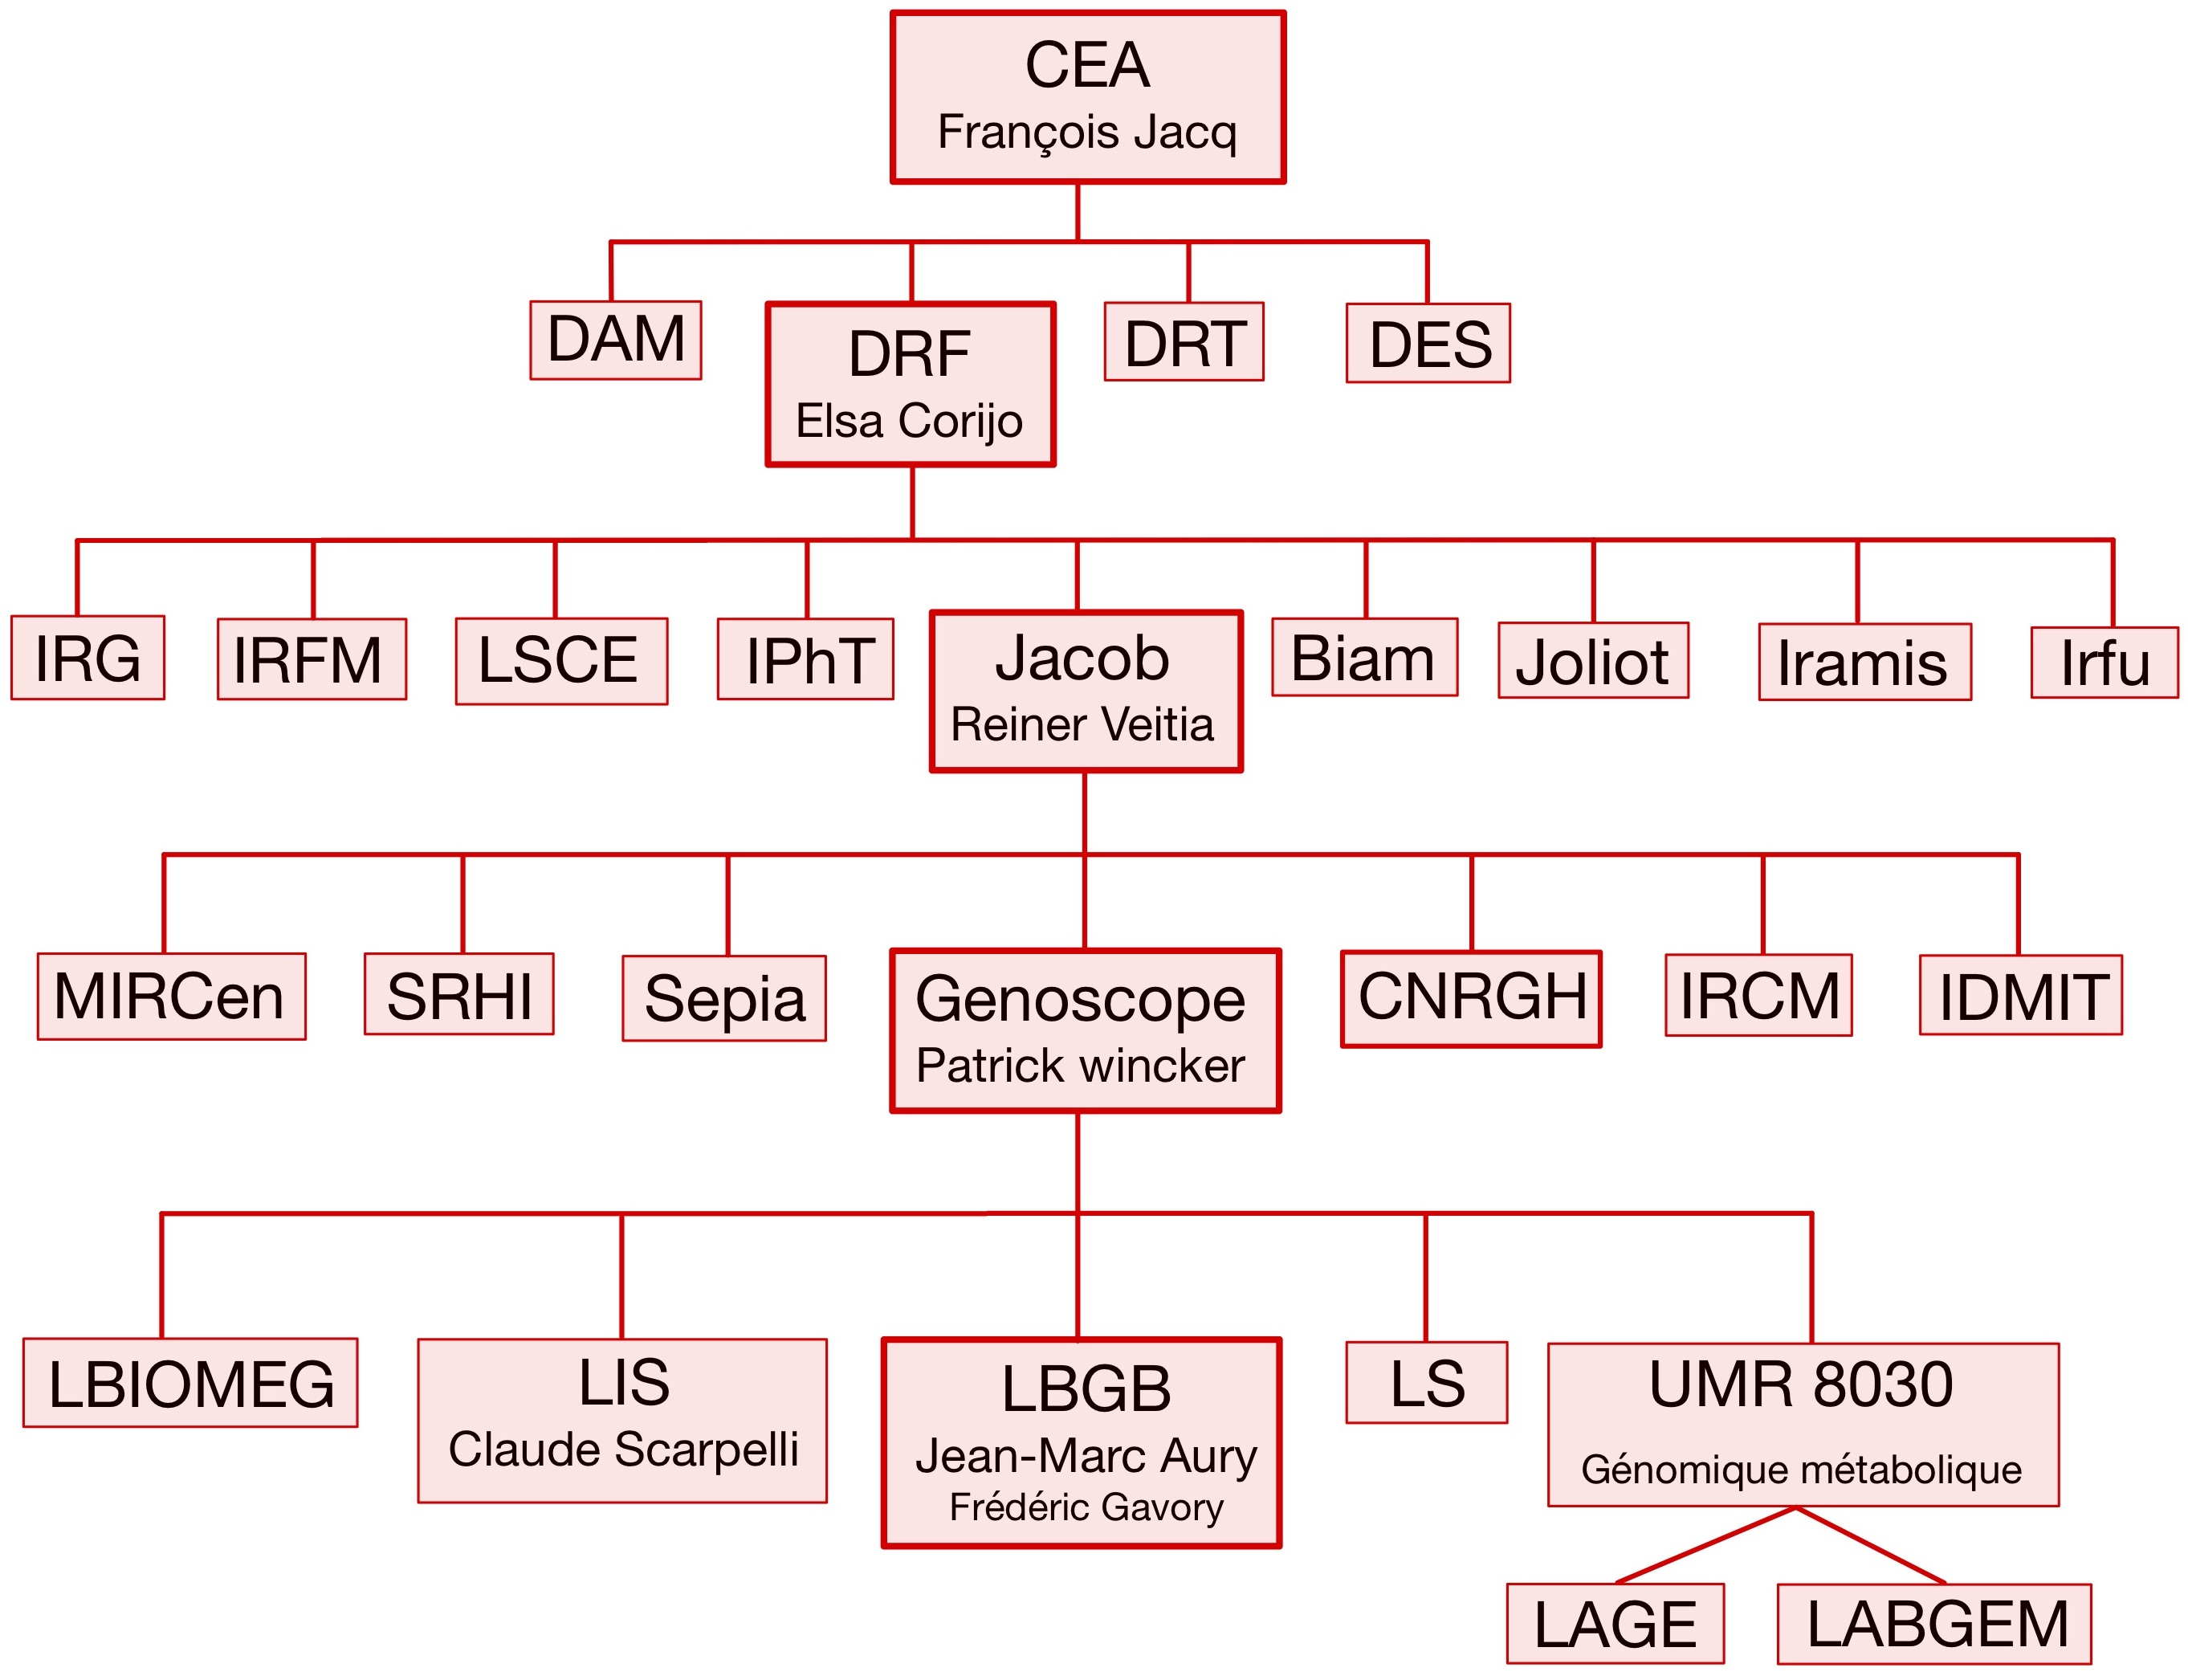
\includegraphics[width=1\textwidth]{img/organigramme.jpg}
    \caption{Organigramme situant l’équipe du LBGB au sein du Genoscope et du CEA}
    \label{organigramme_LBGB}
\end{figure}
\end{minipage} 
\hfill
\begin{minipage}{0.5\textwidth}
    Le Laboratoire de Bioinformatique pour la Génomique et la Biodiversité (\textbf{LBGB}) dirigé par Jean-Marc Aury, fait partie du Genoscope qui est une composante de l'institut François Jacob (\textbf{IBFJ}) de la direction de la recherche fondamentale (\textbf{DRF}) du Commissariat à l'Énergie Atomique et aux Énergies Alternatives (\textbf{CEA}), qui a été fondé le 18 octobre 1945 par Charles de Gaulle. L'intégration du genoscope au CEA a été réalisée en 2007, et en 2017 il devient une composante de l'IBFJ.
\end{minipage}

\subsection{Contexte et missions du LBGB}
Les missions qui sont confiées au LBGB sont : réaliser le contrôle qualité des données de séquences issues des différents séquenceurs, d'effectuer l'assemblage\footnote{Reconstruction d'un génome à partir fragment de ce dernier} des séquences et l'annotation\footnote{Documenter le plus exhaustivement possible les informations de l'assemblage permmettant de prédire la fonction d'une molécule} des génomes, dans l'objectif de mettre à disposition des laboratoires collaborateurs les données avec un premiers niveau da valorisation. Le laboratoire est divisé en plusieurs groupes de travail. Le groupe \emph{production} (dont je fais parti), le groupe \emph{assemblage}, le groupe \emph{annotation} et le groupe \emph{évaluation des technologies de séquençage}.\\

Les missions du groupe de \emph{production} sont de tester des logiciels tiers, de développer et maintenir des scripts utilisant ces logiciels pour gérer efficacement la prise en charge des données en sortie de séquençeur. Cette prise en charge peut répondre à une demande de la production, mais aussi d'autres laboratoires. L'objectif principale est la mise en place et le maintient de pipelines automatisant l'ensemble. Le groupe s'appuie sur un travail de vielle et d'évaluation technologique pour chacune de ses missions. 


\subsection{Présentation du workflow NGS}
\begin{minipage}{0.45\textwidth}
	\begin{figure}[H]
		\centering
		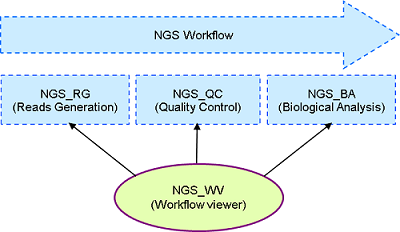
\includegraphics[width=1\textwidth]{img/Workflow.png}
		\caption{\footnotesize{Workflow de génération, de contrôle qualité et d’analyse biologique des fastq}}
		\label{worflow-genoscope}
	\end{figure}
\end{minipage} 
\hfill
\begin{minipage}{0.45\textwidth}
	Le workflow ngs\footnote{\emph{Next Generation Sequencing}} est composé de trois pipelines pour les technologies Illumina, Oxford Nanopore, PacBio. Le premier (ngs\_rg\footnote{\emph{Next Generation Sequencing - reads generation}}), permet la génération des reads\footnote{Lecture d'une séquence par un séquenceur d'un fragments d'ADN}. Le second (ngs\_qc\footnote{\emph{Next Generation Sequencing - quality control}}), permet de réaliser le contrôle qualité des fichiers de séquences. Le dernier (ngs\_ba\footnote{\emph{Next Generation Sequencing - biological analysis}}), permet de faire les analyses biologiques de lot de séquence\footnote{un lot de séquences est une instance de séquences (ou reads) d'un échantillon}. Ces trois pipelines sont automatisés dans le workflow et permmettent de réaliser la distribution des données de séquences par projet, de les trier par échantillons, runs\footnote{séquençage d'un ou plusieurs échantillons sur un séquenceur} et technologies de séquençage. Ils réalisent aussi le nettoyage, l'analyse de ces fichiers et mettent à jour la base de données de référence ngl\footnote{\emph{Next Generation LIMS (Laboratory Information Management System)}}.
\end{minipage} 

\subsection{La technologie MGI}
Le genoscope et le CNRGH\footnote{Centre National de Recherche en Génétique Humaine} ont récement fait l'aquisition de séquenceurs MGI\footnote{Membre du groupe BGI dont les missions sont : R\&D, production et vente d'instruments de séquençage d'ADN, de réactifs et de produits connexes} (2 DNBSEQ-G400 et 1 DNBSEQ-T7).

% \begin{figure}[H]
% 	\centering
% 	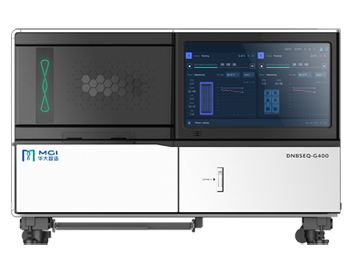
\includegraphics[width=0.3\textwidth]{img/MGI_G400.jpg}
%     \hspace{2.5cm}
%     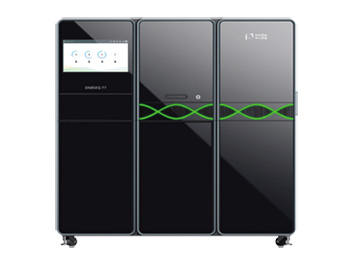
\includegraphics[width=0.3\textwidth]{img/MGI_T7.jpg}
%     \caption{\footnotesize{Sequenceurs DNBSEQ-G400 (à gauche) et \footnotesize (à droite) de MGI \href{https://en.mgi-tech.com/products/}{https://en.mgi-tech.com/products/}}}
% 	\label{seq-MGI}
% \end{figure}

\begin{minipage}{0.45\textwidth}
	\begin{figure}[H]
        \centering
        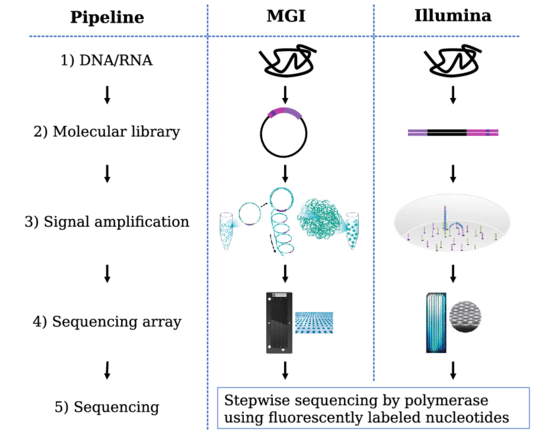
\includegraphics[width=1\textwidth]{img/MGI_vs_Illumina.png}
        \caption{\footnotesize{Différences entre Illumina et MGI de technologie NGS}}
        \label{fig-Illu-vs-MGI}
    \end{figure}
\end{minipage} 
\hfill
\begin{minipage}{0.45\textwidth}
    Il s'agit de séquenceurs à haut débit, dont les principales différences entre MGI et Illumina sont dans la création des librairies et la méthode d'amplification d'ADN. Les librairies sont double brins circulaire pour MGI, alors que pour Illumina elle est double brins linéaire. L'amplification ADN est réalisée en solution et forme des \emph{DNA-nanoballs}\footnote{nanobilles d'ADN générer par la réplication de l'ADN circulaire} pour MGI puis déposée sur la Flowcell\footnote{Lame d'absorbtion des fragment d'ADN et cuve réacteur du séquençage}, alors que pour Illumina elle esr réalisée après immobilisation sur les Flowcell.
\end{minipage}

\begin{table}[H]
\begin{tabular}{ |p{5cm}||r|r|r|r| }
    \hline
    %\multicolumn{5}{|c|}{Sequencers specifications} \\\hline
    & \footnotesize{DNBSEQ-G400} & \footnotesize{DNBSEQ-T7} & \footnotesize{HiSeq 4000} & \footnotesize{NovaSeq 6000} \\\hline\hline
    Max Number of Flow Cells & 2 & 4 & 2 & 2 \\\hline
    Max Lane/Flow Cell & 4 & 1 & 4 & 4 \\\hline
    Run Time & $\sim$ 14-37 h & $\sim$ 20-30 h & $\sim$ 24-84 h & $\sim$ 13-44 h \\\hline
    \textbf{Data ouput/Run} & 0.27-1.4 Tb & 1-6 Tb & 0.9-1.8 Tb & 1-6 Tb \\\hline
    Max Reads/Run & 1.8 billions & 5 billions & 10 billions & 20 billions \\\hline
    Max Read Length & 2 $\times$ 200 bp & 2 $\times$ 150 bp & 2 $\times$ 150 bp & 2 $\times$ 250 bp \\\hline
\end{tabular}
    \caption{Spécification des séquenceurs}
    \label{spe-seq}
\end{table}

%==============================================================================%
%=============================== Objectifs ====================================%
\section{Objectifs}
L'objectif principal de ma mission est la mise en place d'un workflow pour les séquenceurs de MGI. Plus précissément il s'agira de créer un pipeline de génération de reads (ngs\_rg\_mgi\footnote{\emph{Next Generation Sequencing - reads generation - mgi}) et un pour le contrôle qualité (ngs\_qc\_mgi\footnote{\emph{Next Generation Sequencing - quality control - mgi}). Le workflow devra créer et mettre à jour l'état des runs et des \emph{lanes}\footnote{pistes présentes sur la \emph{flow cell}} dans ngl, réaliser le contrôle qualité des fichiers de séquence, au format fastq, obtenu après démultiplexage\footnote{Séparation des différents \emph{reads} d'une \emph{lane} en fonction de l'index d'échantillon} des runs. Il devra mettre à jour l'avancement du traitement d'un run dans ngl, en y indiquant les statistiques obtenu lors du démultiplexage, les résultats des contrôles qualités, etc. Puisque l'objectif est d'obtenir un premier niveau de valorisation des fichier de séquences, permettant aux autres groupes (\emph{assemblage}, \emph{anotation}) de prendre en charge ses fichier avant de les mettrent à disposition des laboratoires collaborateurs.


Je devrais également, rechercher et réaliser des évaluations de nouveaux outils pour les différents pipelines des différentes technologies de séquençage. En vue d'un potentiel ajout d'outils ou de remplacement d'outils. Il sera donc necessaire de maintenir les pipelines des différentes technologies de séquençage en conséquence.


%==============================================================================%
%================================ Méthodes ====================================%
\section{Matériels et Méthodes}

La Genoscope possède 7 clusters de calucls pour la \emph{production} sur le serveur \emph{inti}, ces derniers disposent de 16 coeurs et de 257 Go d'espace de stockage. L'accès à l'utilisation des clusters est réalisé par le logiciel Slurm\footnote{Logiciel open source d'ordonnancement des tâches informatiques}. Il dispose également de sa propre base de données de référence (ngl). La gestion et le suivi du développememnt informatique est réalisé par le système Jira\footnote{Logiciel de gestion de projet, d'incidents et de suivi de bugs}. 
L'écriture du workflow des pipelines pour les séquenceurs MGI sera réalisée dans le langage de programmation Perl. L'utilisation de ce langage est rendu necessaire pour des raisons historique du laboratoire, puisque de nombreuses librairies et modules qui seront à utiliser dans l'écriture des pipelines sont écrits en Perl. Le workflow pour MGI s'appuirera sur le workflow d'Illumina qui est totalement implémenté en Perl. 

C'est pour toutes ces raisons qu'il m'a été nécessaire d'apprendre à coder en Perl en réalisant un programme permettant de faire des analyses statistiques élémentaires sur des fichiers fastq. Tel que le taux de GC, la moyenne du score de la qualité, ainsi que plusieurs autres métriques. Le programme est capable de gérer les fichiers fastq issue de séquençage \emph{single end\footnote{Lecture dans un seul sens des reads par le séquenceur}} et \emph{paired end\footnote{Lecture dans les deux sens des reads par le séquenceur}}. Cela m'a permis de prendre en main les modules utilisés pour les différents pipelines déja en place, notament pour le pipelines d'llumina. De plus cela m'a permi de prendre en main de l'environement de travail, l'utilisation du lancement de job sur les noeuds de calculs et l'utilisation des modules utilisés pour le workflow d'llumina\\

Une première évaluation d'outils a également été efféctuée en vu du remplacement de bcl2fastq par bcl-convert. Il s'agit de deux logiciels de génération de fichiers fastq et de démultiplexage qui sont développés et commercialisés par Illumina.

Dans un premier temps, il a été nécessaire de déterminer les conditions optimales (temps total rapide, pourcentage d'utilisation cpu\footnote{Central Processing Unit (unité centrale de traitement, en français)} maximum) en fonction des ressource disponible sur les clusters de la \emph{prodution} (16 coeurs maximum) du nouveau serveur (\emph{inti}), pour bcl2fasq dans l'objectif de pouvoir comparer les performances des deux logiciels dans les mêmes conditions. Les conditions optimales sont déterminées en fonction des paramètres suivant de bcl2fatq : 
\begin{itemize}
    \item[•] \texttt{r} : nombre de \emph{threads\footnote{Processus : instructions du langage machine d'un processeur.}} accordé pour la décompréssion et la lecture des \emph{Bases Calls\footnote{Fichier d'attribution des bases nucléiques en fonction des pics du chromatogramme lors du séquençage}}
    \item[•] \texttt{p} : conversion des \emph{Bases Calls} en fastq
    \item[•] \texttt{w} : écriture et compréssion des fichier fastq
\end{itemize}

Tous ces tests ont été  réalisés sur le même noeud de calcul, dans l'objectif de minimiser les biais. La comparaison est effectuée sur le temps total de génération des fastq et le démultiplexage, ainsi que le temps cpu et le pourcentage d'utilisation des cpu.

%==============================================================================%
%================================ Resultats ===================================%
\section{Résultats des évaluations de bcl2fastq et bcl-convert}

\subsection{Détermination des meilleurs paramètres pour bcl2fastq}
Après avoir effectué différentes combinaisons des paramètres, nous avons mis en évidence que la variation du paramètre \texttt{r} et \texttt{w} en fixant le paramètre \texttt{p}, n'apportait pas de différences significatives pour le temps total d'exécution, le temps cpu ou le pourcentage d'utilisation cpu, comme on peut l'observé sur la figure \ref{barplot-param}. 

\begin{figure}[H]
    \centering
    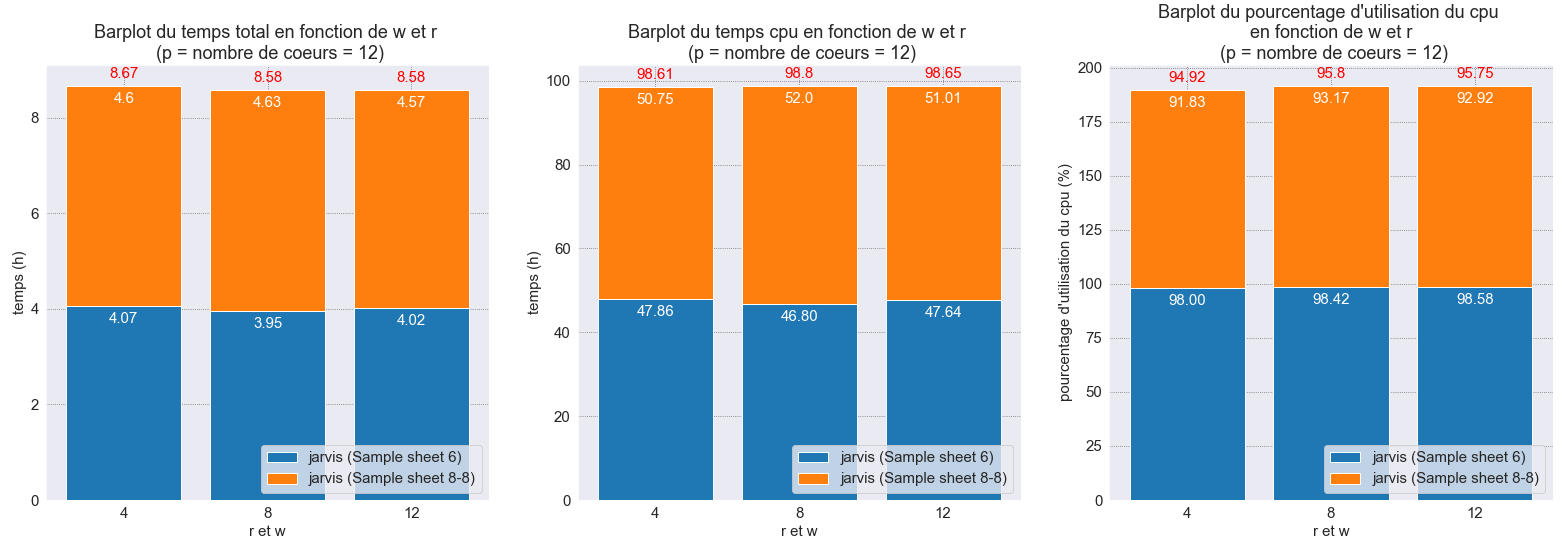
\includegraphics[width=1\textwidth]{img/barplot_cum_jarvis2.png}
    \caption{\footnotesize{Digrammes en bâtons du temps total d'éxécution (à gauche), temps cpu (au milieu) et du pourcentage d'utilisation des cpu (à droite)}}
    \label{barplot-param}
\end{figure} 
Il y a deux \emph{sample sheet}, car le nombre de bases considérés des \emph{reads index} entre les \emph{lanes} est différent, obligeant à réaliser deux appels différents au logiciel pour générer les fastq et le démultiplexage.

\subsection{Comparaison entre bcl2fastq et bcl-convert}
Nous avons donc fait varier les paramètres \texttt{p}, \texttt{r} et \texttt{w} de manière à ce que chacun des paramètre soit égale au nombre de coeurs accordés aux deux logiciels. On observe bien, sur la figure \ref{fig-total-time}, que plus on augmente le nombre de coeurs pour chacun des logiciels (et donc le nombre de \emph{threads} pour \texttt{p}, \texttt{r} et \texttt{w}) plus la génération des fastq et le démultiplexage est rapide. De plus on remarque que bcl-convert permet de réduire le temps d'environs 1/3 par rapport à bcl2fatq. 

\begin{figure}[H]
    \centering
    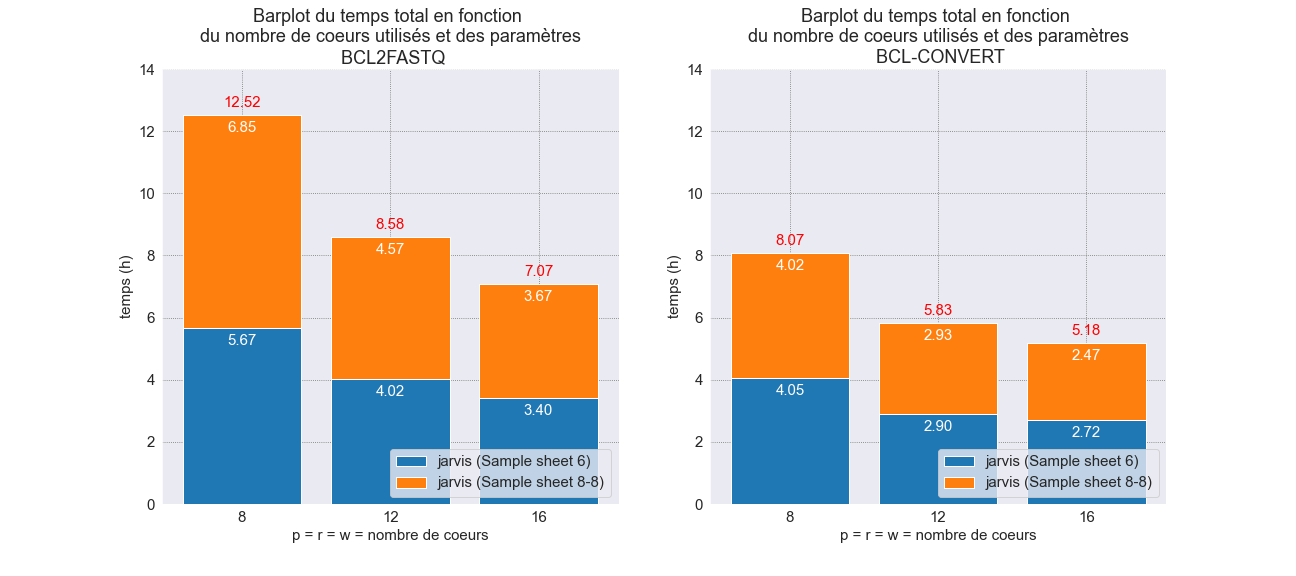
\includegraphics[width=1\textwidth]{img/barplot_total_time_comp.png}
    \caption{\footnotesize{Temps total de génération des fastq pour bcl2fastq et bcl-convert}}
    \label{fig-total-time}
\end{figure}


 
%==============================================================================%
%======================== Conclusion et perspectives ==========================%
\section{Perspectives}
Concernant les perspectives de bcl-convert il reste à réaliser un cahier des charges référençant tous les changements à effectuer dans les différents pipeplines pour la mise à jour de bcl2fastq vers bcl-convert. Ce cahier des charges prendra en compte le changement d'arborescence des fichiers de sortie entre les deux logiciels, ainsi toutes les modifications à effectuer dans les différents pipelines pour permettre le bon fonctionnement des workflow. Dû à la pression actuelle autour de la technologie MGI, c'est un autre développeur qui se chargera de suivre ce cahier des charges et de réaliser les modifications.\\

Concernant le workflow de MGI, il nous faut dans un premier temps déterminer les outils et méthodes necessaires (utilisation de ceux du workflow d'Illumina ou de nouveaux). Une fois ceci déterminé il restera à écrire les deux pipelines, celui de génération de reads (ngs\_rg\_mgi) et celui de contrôle qualité (ngs\_rg\_mgi). L'objectif sur le long terme est d'arriver à un workflow totalment automatisé, comme celui d'Illumina.\\

Il y a aussi l'évaluation d'autres outils utiles pour les pipelines, comme l'évaluation d'outils de \emph{trimming}, \emph{filtering}, d'assignation taxonomique, ect.

\newpage
\subsection{diagramme de gantt}
\begin{figure}[H]
    \centering
    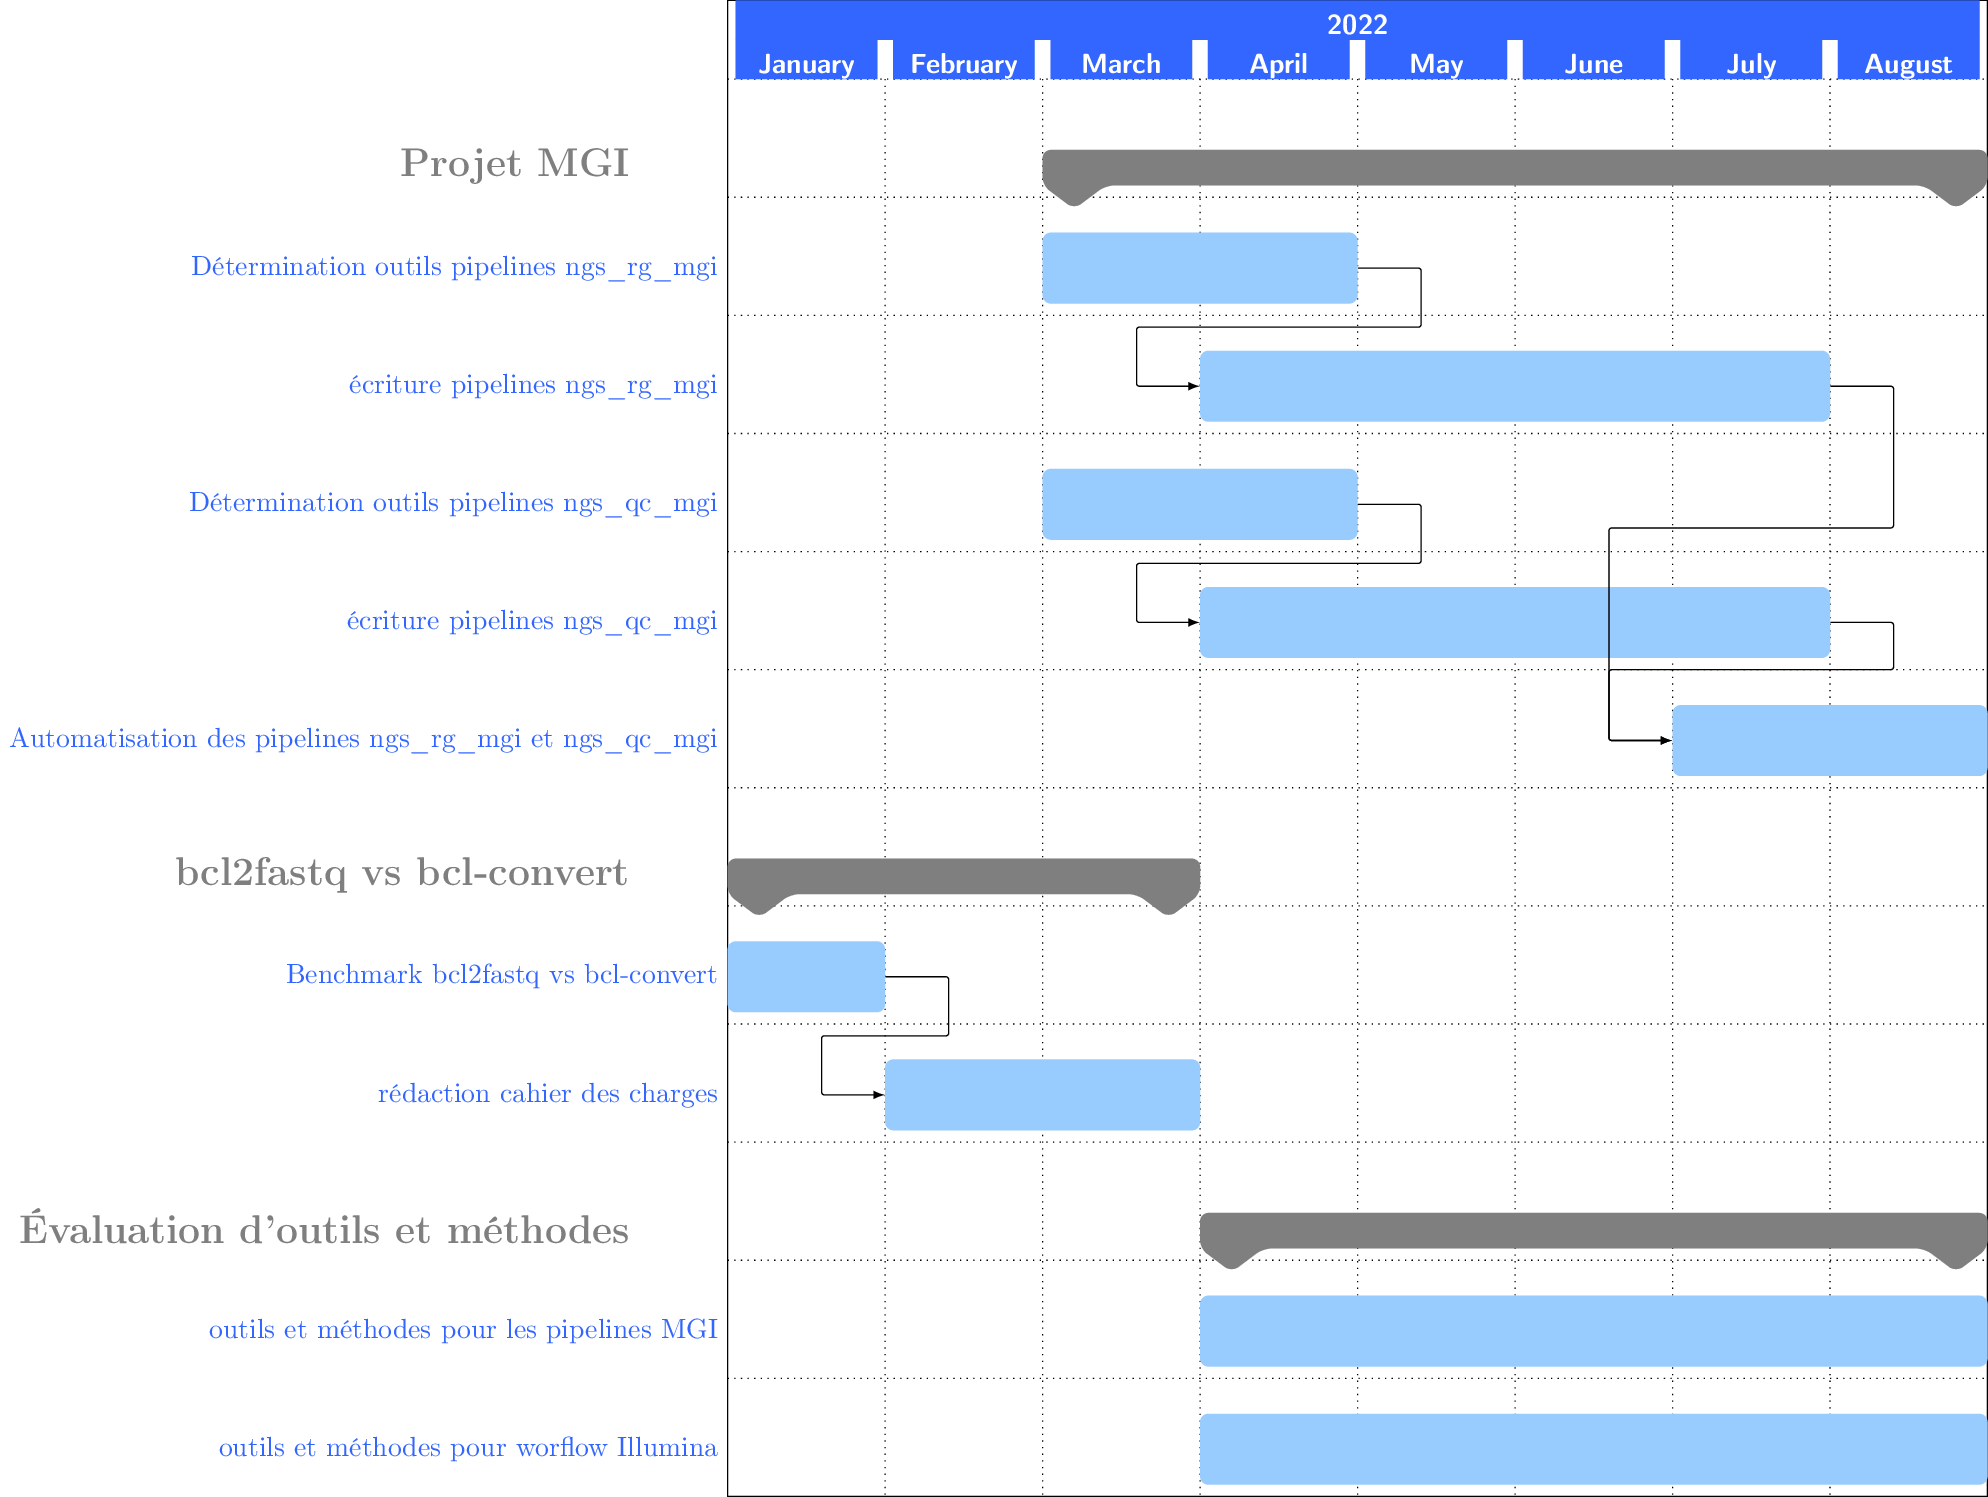
\includegraphics[width=1\textwidth]{digramme_gant/diag_gantt.png}
    \caption{Digramme de gantt des différents projets et missions}
    \label{diag-gantt}
\end{figure}